\addtocounter{section}{1}
\subsection{Task 1.1: Parsing}

%task 1.1.1
\subsubsection{}
Even with unlimited lookahead, with a finite set of regular languages, an LL approach can still be stuck recursing with a left-recursive grammar.

%task 1.1.2
\subsubsection{}
We start with the grammar:
\begin{description}
 \item[] $F \rightarrow f I v A w S x$
 \item[] $A \rightarrow P$
 \item[] $P \rightarrow P I | \epsilon$
 \item[] $S \rightarrow S s | s$
 \item[] $I \rightarrow i$
\end{description}
The productions
\begin{description}
 \item[] $S \rightarrow S s | s$
\end{description}
and
\begin{description}
 \item[] $P \rightarrow P I | \epsilon$
\end{description}
are left-recursive.
This is solved by splitting them into two more productions:
\begin{description}
 \item[] $S \rightarrow sS'$
 \item[] $S'\rightarrow \epsilon | s S'$
 \item[] $P \rightarrow \epsilon P'$
 \item[] $P'\rightarrow \epsilon | I P'$
\end{description}
So we now have the grammar:
\begin{enumerate}
 \item $F  \rightarrow f I v A w S x$
 \item $A  \rightarrow P$
 \item $S  \rightarrow sS'$
 \item $S' \rightarrow \epsilon | s S'$
 \item $P  \rightarrow \epsilon P'$
 \item $P' \rightarrow \epsilon | I P'$
 \item $I  \rightarrow i$
%\end{description}
\end{enumerate}

%task 1.1.3
\subsubsection{}
Nullable:
\begin{description}
 \item[] P'
 \item[] S'
\end{description}
See Table \ref{table:sets} and \ref{table:ptable}.\\
For the FIRST set, you add a terminal if the symbol is a terminal. If the symbol is a non-terminal, add the FIRST set from this non-terminal, minus $\epsilon$. Recurse down through non-terminals until you hit a terminal. If $\epsilon$ is in all, add $\epsilon$.\\
For the FOLLOW set, start by adding the marker for end of input (\$) to the start symbol. For productions of type $X \rightarrow aYc$ where Y is a non-terminal, add FIRST(c) minus $\epsilon$ to FOLLOW(Y). If v is nullable, or a production $X \rightarrow aY$ exists, add FOLLOW(X) to FOLLOW(Y).

\begin{table}
 \centering
  \begin{tabular}{| c | c | c |}
      \hline
      \textsc{Production} & \textsc{FIRST} & \textsc{FOLLOW}     \\ \hline
       F  & \{ f \} & \{ \$ \} \\ \hline
       A  & \{ $\epsilon$, i,  \} & \{ w \} \\ \hline
       P  & \{ $\epsilon$, i \} & \{ w \} \\ \hline
       P' & \{ $\epsilon$, i \} & \{ w \} \\ \hline
       S  & \{ s \} & \{ x \} \\ \hline
       S' & \{ s, $\epsilon$ \} & \{ x \} \\ \hline
       I  & \{ i \} & \{ v \} \\ \hline
  \end{tabular}
 \caption{First and follow sets}
  \label{table:sets}
\end{table}

\begin{table}
 \centering
  \begin{tabular}{| c | c | c | c | c | c | c | c |}
      \hline
                   & f & i & v & w & s & x & \$ \\ \hline
       \textsc{F}  & 1 & - & - & - & - & - & -  \\ \hline
       \textsc{A}  & - & 2 & - & 2 & - & - & -  \\ \hline 
       \textsc{S}  & - & - & - & - & 3 & - & -  \\ \hline
       \textsc{S'} & - & - & - & - & 4 & 4 & -  \\ \hline
       \textsc{P}  & - & 5 & - & 5 & - & - & -  \\ \hline 
       \textsc{P'} & - & 6 & - & 6 & - & - & -  \\ \hline
       \textsc{I}  & - & 7 & - & - & - & - & -  \\ \hline
  \end{tabular}
 \caption{Parse table}
  \label{table:ptable}
\end{table}

\subsubsection{}
\begin{lstlisting}

Stack                   Input                        Rule (production)
F, $ 
f I v A w S x, $        f i v i i i i w s s s x      F
I v A w S x, $          i v i i i i w s s s x        I
i v A w S x, $          i v i i i i w s s s x        elim
v A w S x, $            v i i i i w s s s x          elim
A w S x, $              i i i i w s s s x            A
P w S x, $              i i i i w s s s x            P
P' w S x, $             i i i i w s s s x            P'
IP' w S x, $            i i i i w s s s x            I
iP' w S x, $            i i i i w s s s x            elim
P' w S x, $             i i i w s s s x              P'
IP' w S x, $            i i i w s s s x              I
iP' w S x, $            i i i w s s s x              elim
P' w S x, $             i i w s s s x                P'
IP' w S x, $            i i w s s s x                I
iP' w S x, $            i i w s s s x                elim
P' w S x, $             i w s s s x                  P'
IP' w S x, $            i w s s s x                  I
iP' w S x, $            i w s s s x                  elim
P' w S x, $             w s s s x                    P' -> epsilon
w S x, $                w s s s x                    elim
S x, $                  s s s x                      S
sS' x, $                s s s x                      elim
S' x, $                 s s x                        S'
sS' x, $                s s x                        elim
S' x, $                 s x                          S'
sS' x, $                s x                          elim
S' x, $                 x                            S' -> epsilon
x, $                    x                            elim
$                                                    ACCEPTED!

\end{lstlisting}
\begin{figure}[here]
	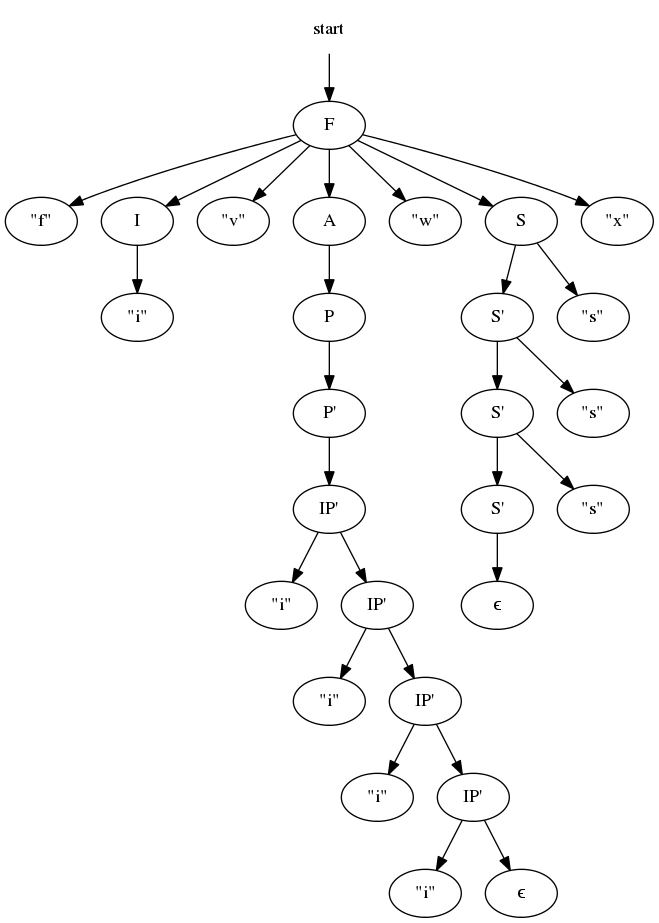
\includegraphics[width=0.9\textwidth]{img/graph.png}
	\caption{Parse tree for Task 1.1.4. Did a shortcut on IP' for readability reasons.}
	 \label{fig:parsetree}
\end{figure}
See Figure \ref{fig:parsetree}.
\subsubsection{}

\begin{lstlisting}
Stack                   Input                       Rule
$                       f i v i i i i w s s s x
f, $                    i v i i i i w s s s x       SHIFT
f i, $                  v i i i i w s s s x         SHIFT
f I, $                  v i i i i w s s s x         REDUCE
f I v, $                i i i i w s s s x           SHIFT
f I v P, $              i i i i w s s s x           REDUCE
f I v Pi, $             i i i w s s s x             SHIFT
f I v PI, $             i i i w s s s x             REDUCE
f I v P, $              i i i w s s s x             REDUCE
f I v Pi, $             i i w s s s x               SHIFT
f I v PI, $             i i w s s s x               REDUCE
f I v P, $              i i w s s s x               REDUCE
f I v Pi, $             i w s s s x                 SHIFT
f I v PI, $             i w s s s x                 REDUCE
f I v P, $              i w s s s x                 REDUCE
f I v Pi, $             w s s s x                   SHIFT
f I v PI, $             w s s s x                   REDUCE
f I v P, $              w s s s x                   REDUCE
f I v A, $              w s s s x                   REDUCE
f I v A w, $            s s s x                     SHIFT
f I v A w s, $          s s x                       SHIFT
f I v A w S, $          s s x                       REDUCE
f I v A w S s, $        s x                         SHIFT   
f I v A w S, $          s x                         REDUCE
f I v A w S s, $        x                           SHIFT   
f I v A w S, $          x                           REDUCE
f I v A w S x, $                                    SHIFT   
F, $                                                REDUCE
$                                                   ACCEPTED
\end{lstlisting}


